\documentclass[english]{lni}
\usepackage[utf8]{inputenc}
\usepackage[T1]{fontenc}
\usepackage{graphicx}
\usepackage{longtable}
\usepackage{listings}
%\usepackage[ngerman]{babel}
\usepackage{float}
%\usepackage{wrapfig}
\usepackage{soul}
\usepackage{amssymb}
\usepackage{hyperref}
\usepackage[utf8]{inputenc}
\usepackage[T1]{fontenc}
\usepackage{fixltx2e}
\usepackage{graphicx}
\usepackage{longtable}
\usepackage{float}
\usepackage{wrapfig}
\usepackage{soul}
\usepackage{textcomp}
\usepackage{marvosym}
\usepackage{wasysym}
\usepackage{latexsym}
\usepackage{amssymb}
\usepackage{hyperref}
\tolerance=1000
\providecommand{\alert}[1]{\textbf{#1}}

\title{Academic impact of DBpedia}
\author{Marcus Nitzschke}
\date{14.06.2012}
\hypersetup{
  pdfkeywords={},
  pdfsubject={},
  pdfcreator={Emacs Org-mode version 7.8.08}}

\begin{document}

\maketitle


\begin{abstract} 
There is an extensive collection of academic papers and presentations for the
Wikipedia project available. This enables one to analyze the evolution of such
projects over the years from the beginning. The goal of this paper is to create a
similar collection for the DBpedia project. With this base there will be
introduced several analyses and a comparison to the Wikipedia project.
\end{abstract}

\section{Introduction}
\label{sec-1}

  In 2011 there was a large survey to collect journal articles and conference
  paper concerning the Wikipedia project. The findings of this survey were published
  and partly analyzed\footnote{\href{http://en.wikipedia.org/wiki/Wikipedia:Academic_studies_of_Wikipedia}{http://en.wikipedia.org/wiki/Wikipedia:Academic\_studies\_of\_Wikipedia} }. Such an analysis showed that the number of
  conference paper decreased constantly from five years after the founding
  while the number of journal articles still grows.

  A similar analysis for the DBpedia project is the goal of this paper. DBpedia
  extracts structured content from Wikipedia and republishs this content in a
  semantically understandable way. This leads to one of the most important datasets in the
  \emph{Linked Open Data} cloud\footnote{\href{http://richard.cyganiak.de/2007/10/lod/}{http://richard.cyganiak.de/2007/10/lod/} }. The DBpedia project was founded in 2007.
\subsection{Important Conferences/Journals}
\label{sec-1-1}

  The following listing introduces the abbreviations of the main conferences and
  main journals named in this paper.
\begin{itemize}
\item \textbf{ESWC} -- \emph{Extended Semantic Web Conference}
\item \textbf{ISWC} -- \emph{International Semantic Web Conference}
\item \textbf{LDOW} -- \emph{Linked Data on the Web}
\item \textbf{WWW} -- \emph{World Wide Web Conference}
\item \textbf{J. Web Sem.} -- \emph{Journal of Web Semantics}
\item \textbf{SWJ} -- \emph{Semantic Web Journal}
\end{itemize}
\section{Methods}
\label{sec-2}

  This chapter describes which data sources were used and how the informations
  were retrieved and processed. This should lighten the process of replication
  for further examinations.
\subsection{Data retrieval}
\label{sec-2-1}

   The process of data retrieval included four sources. Table
   \ref{tab:datenquellen} gives an overview of these sources and the resulting
   number of publications.
\begin{table}[htb]
\caption{Overview of data sources} \label{tab:datenquellen}
\begin{center}
\begin{tabular}{lr}
\hline
 source                          &  results  \\
\hline
 Google Scholar                  &       84  \\
 Arnetminer                      &       54  \\
 Semantic Web Conference Corpus  &       49  \\
 manually                        &        4  \\
\hline
\end{tabular}
\end{center}
\end{table}

   The main criteria was that the term ``dbpedia'' occurs in the title
   or -- if supported by the source -- the abstract of the
   publication. Later the total amount was reduced to only match
   conference papers and journal articles which were all peer
   reviewed.

   The following listing describes how the informations of the
   different data sources were retrieved.
\begin{itemize}
\item \textbf{Google Scholar}

     Google Scholar\footnote{\href{http://scholar.google.com/}{http://scholar.google.com/} } allows to search a multiplicity of academic
     publications. The search was limited because the intent of this paper is to
     collect only the most relevant publications concerning DBpedia. The search
     term \texttt{allintitle:dbpedia} limited the total number of results to that
     containing ``dbpedia'' in their title. This search produced 84 results at the
     moment of writing (06/2012).
\item \textbf{Arnetminer}

     Arnetminer\footnote{\href{http://arnetminer.org/}{http://arnetminer.org/} } is a search engine which extends the collection of
     academic documents with informations about authors, conferences or
     journals. These informations linked together should enable a complete view
     of the data. In comparison to Google Scholar this also allows larger search
     possibilities. Besides the frontend search Arnetminer also provides a REST
     interface\footnote{\href{http://arnetminer.org/RESTful_service}{http://arnetminer.org/RESTful\_service} }. So it is possible to search the publications by title. For
     better processing the retrieved data was converted from JSON to Bibtex by a
     small script\footnote{\href{https://raw.github.com/kenda/dbpedia_impact/master/scripts/get_arnetminer.py}{https://raw.github.com/kenda/dbpedia\_impact/master/scripts/get\_arnetminer.py} }.
\item \textbf{Semantic Web Conference Corpus}

     The Semantic Web Conference Corpus\footnote{\href{http://data.semanticweb.org}{http://data.semanticweb.org} } provides numerous informations about
     conferences and the presented talks belonging to the Semantic Web
     topic. This site also offers a SPARQL endpoint which was used to get the
     relevant publications for this paper. The query retrieved all publications
     with the term ``dbpedia'' in the title or in the abstract. A script\footnote{\href{https://raw.github.com/kenda/dbpedia_impact/master/scripts/get_semweb_org.sh}{https://raw.github.com/kenda/dbpedia\_impact/master/scripts/get\_semweb\_org.sh} } got
     the resulting URIs and scraped the corresponding html view for the Bibtex
     representation of the entry.
\item \textbf{manually}

     The data sources listed so far could not cover all important journals like
     the \emph{Semantic Web Journal} (SWJ). That's why a part of the results was
     collected manually. In case of the SWJ the underlying search term executed by a Google
     search was \texttt{dbpedia site:semantic-web-journal.net/content}. This means that all published research papers by the SWJ were
     searched by the term ``dbpedia''. The resulting pages were reviewed so that the
     term only occured in the title or abstract and not in a review comment for example.
\end{itemize}
\subsection{Data processing}
\label{sec-2-2}

   To ensure a structured organization and analysis of the collected data a
   reference management software, namely Zotero\footnote{\href{http://www.zotero.org/}{http://www.zotero.org/} }, was used. This solution
   has numerous advantages, for example a Bibtex importer and an easy possibility to import
   results from Google Scholar via a browser plugin.

   With the aid of Zotero the data processing first solved duplicates between
   the publications. This step reduced the total number of data entries from 191
   to 130. Six further entries dropped out because of the type of publication,
   e.g. theses or technical reports, which are not in the scope of this
   paper. The second step was to complete lacking data fields like the
   publication date or conference names.

   The cleaned data was exported from the Zotero database to the csv format by a
   SQL script\footnote{\href{https://raw.github.com/kenda/dbpedia_impact/master/scripts/zotero_query.sql}{https://raw.github.com/kenda/dbpedia\_impact/master/scripts/zotero\_query.sql} }. This csv data is the base for the analyses which are done by
   Gnu R\footnote{\href{http://www.r-project.org/}{http://www.r-project.org/} }. The main analyses provided in this paper are:
\begin{itemize}
\item total number of journal articles / conference paper by year
\item total number of journal articles / conference paper by journal/conference
\end{itemize}
\section{Results}
\label{sec-3}

  The results contains the different analyses in the period between 2007
  and 2012. Because this paper was written in June 2012 there is a lack of
  publications for this year. Especially conferences which are mostly held in the
  second half of the year are lacking, e.g. ISWC.
\subsection{Analysis 1}
\label{sec-3-1}

   The first analysis shown in Figure \ref{fig:auswertung1} plots the total
   number of publications by year. This is the analogical visualization of the
   Wikipedia analysis.



\begin{figure}[htb]
\centering
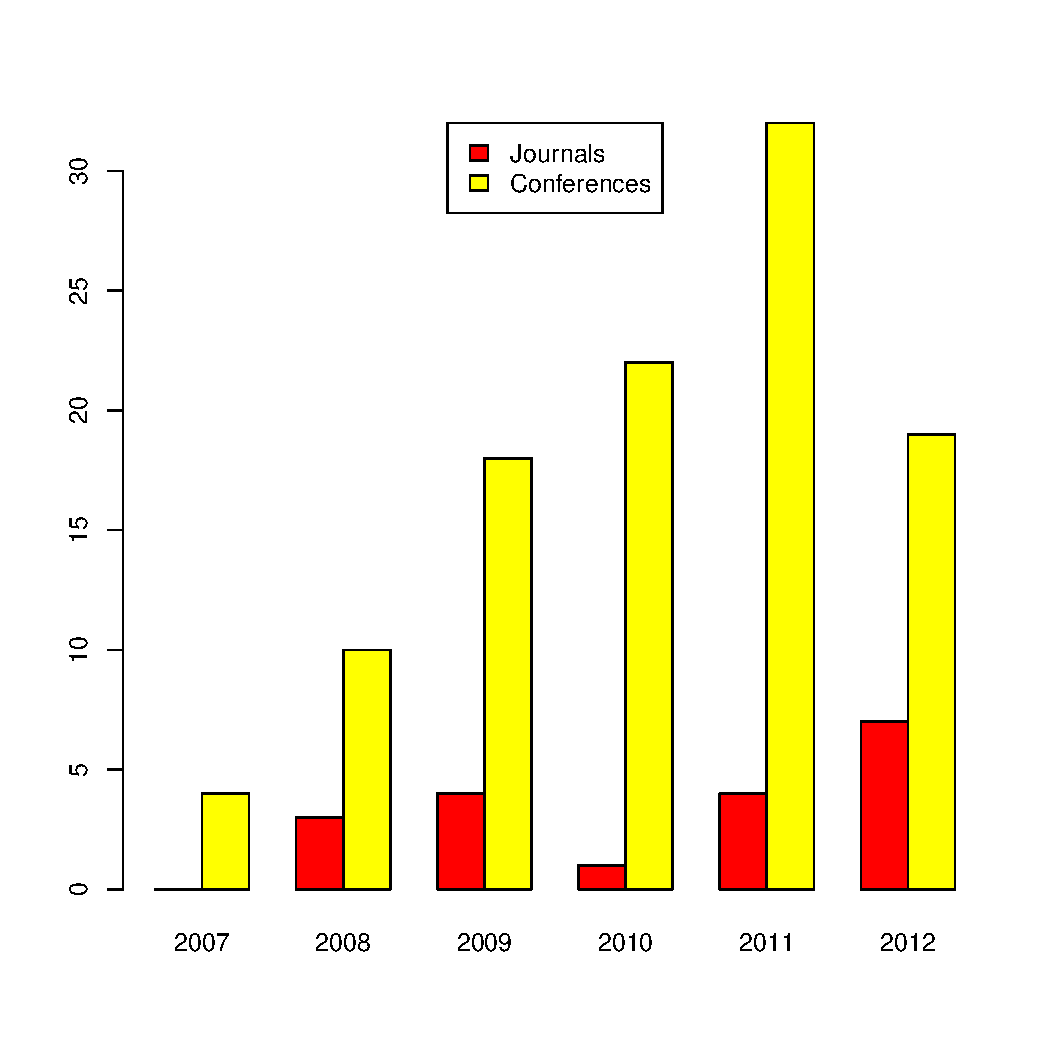
\includegraphics[width=0.6\textwidth]{auswertung1.pdf}
\caption{\label{fig:auswertung1}barplot visualizing total number of publications by year}
\end{figure}

   The barplot shows a minimum number of publications in 2007 of zero and four
   for the journals and conferences respectively. The maximum number of journals
   is already reached in 2012 with seven. The maximum number of conference
   papers was reached in 2011 with 32. But it seems like this number will be
   exceeded in 2012.\\ There is an obvious trend that the number of conference
   papers is constantly growing. The trend of the journal articles is not that
   obvious because there is an outlier in 2010. But this fact is owed to the
   small number of journal articles in general. If we suppose that the number of
   journal articles is normal distributed the value of 2010 is still in the 95\%
   confidence interval [1.19;5.14].\\ The reason why the number of conference
   papers is that greater than the number of journal articles was already
   covered by the Wikipedia analysis. ``Journals are not the norm in
   CS/HCI research. Knowledge is shared through conferences, not journals.''
   \cite{wiki} they explain. But there are opposite areas of research like the life sciences where
   journals have a higher relevance.
\subsection{Analysis 2}
\label{sec-3-2}

   The second analysis goes into the details of the journals and conferences. It
   plots the total number of publications by the specific journal or conference
   if there are at least two publications.
   


\begin{figure}[htb]
\centering
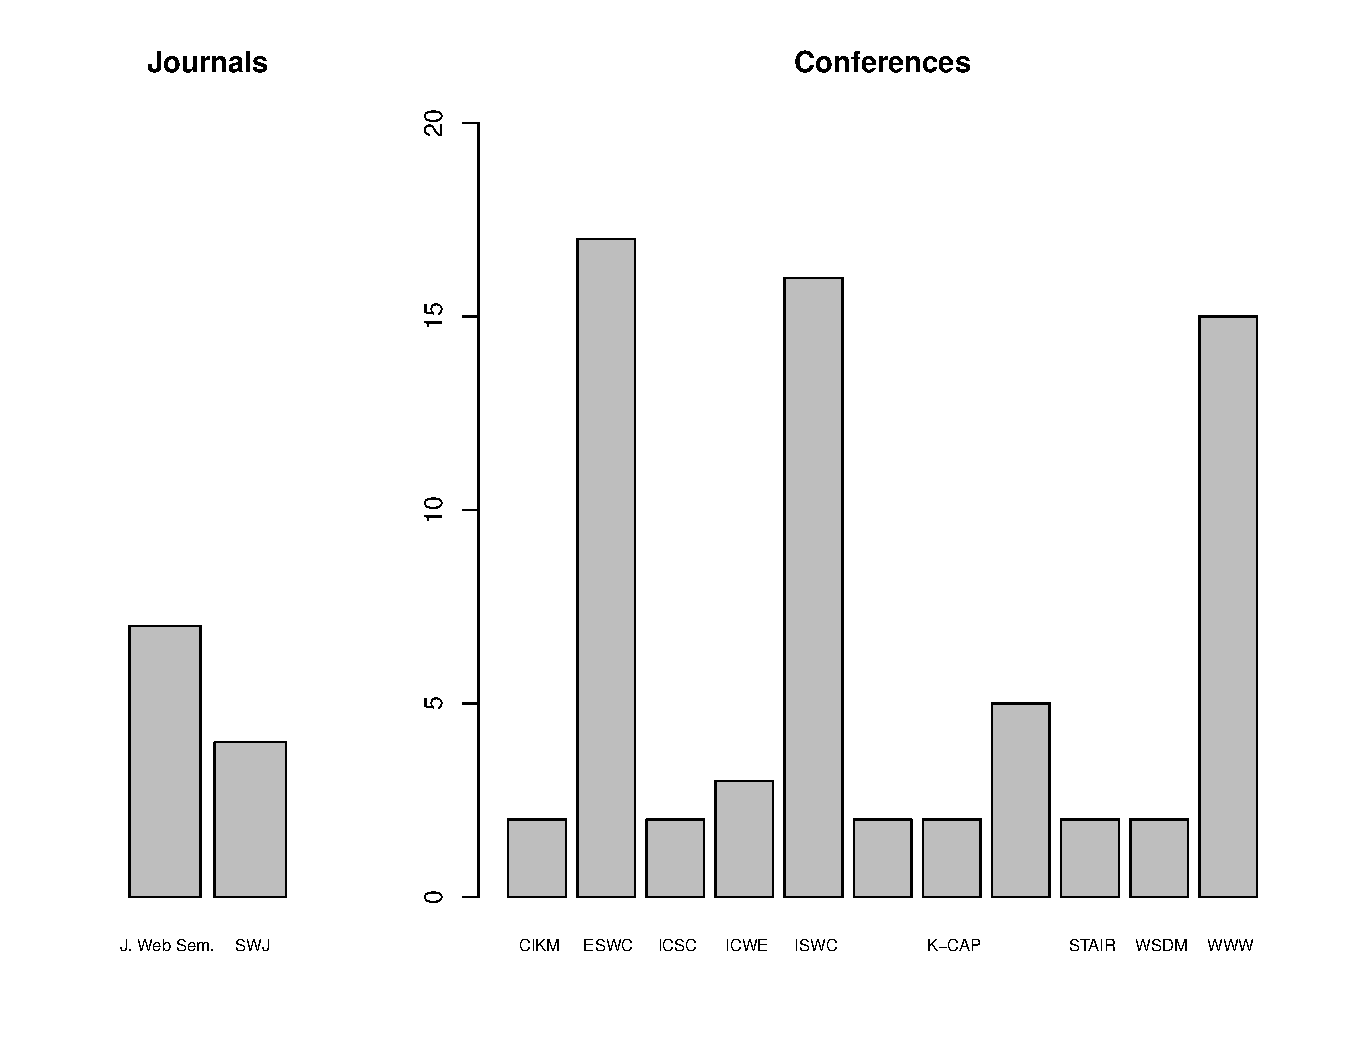
\includegraphics[height=0.8\textwidth]{auswertung2.pdf}
\caption{\label{fig:auswertung2}barplot visualizing total number of publications $n$ by conference/journal with $n > 1$}
\end{figure}

   Figure \ref{fig:auswertung2} illustrates that there are two journals which published
   more than one article related to DBpedia. The \emph{Journal of Web Semantics}
   published seven articles, the \emph{Semantic Web Journal} four articles. The
   second plot shows that there are three major conferences where DBpedia
   mattered since 2007. The most papers were published at \emph{ESWC} with a number
   of 17. \emph{ISWC} and \emph{WWW} published 16 and 15 papers, respectively. It follows
   a gap of 10 to the \emph{LDOW} conference with five published papers. This plot
   assumes the \emph{ISWC/ASWC} as a seperate conference. Otherwise \emph{ISWC} would have
   two additional publications and therefore 18 overall.
   
\subsection{Analysis 3}
\label{sec-3-3}


   Table \ref{tab:vergleich} shows the importance of DBpedia at the major
   conferences in 2011. The table breaks the total number of publications at the
   conferences down to the number of publications where the term ``dbpedia''
   occured somewhere in the paper and the number of publications where the term
   occured in the title or abstract.

\begin{table}[htb]
\caption{\centering Compared number of publications at ESWC, ISWC, WWW in 2011 \\\hspace{0.4cm}dbpedia$_{1}$ representing the occurence of ``dbpedia'' in full paper \\\hspace{1.05cm}dbpedia$_{2}$ representing the occurence of ``dbpedia'' in title or abstract} \label{tab:vergleich}
\begin{center}
\begin{tabular}{llll}
\hline
                &  ESWC (\%)  &  ISWC (\%)  &  WWW (\%)   \\
\hline
 total          &  57 (100)   &  163 (100)  &  220 (100)  \\
 dbpedia$_{1}$  &  N/A        &  14 (8.59)  &  12 (5.45)  \\
 dbpedia$_{2}$  &  4 (7.02)   &  9 (5.52)   &  1 (0.45)   \\
\hline
\end{tabular}
\end{center}
\end{table}


   Therefore DBpedia was mentioned in 8.59\% and 5.45\% of the publications at
   ISWC and WWW somewhere in the paper. The highest rate of the dbpedia$_{2}$
   criteria was reached by ESWC with 7.02\% and a number of four papers. There
   were five more papers at ISWC, however this led to a lower percentage
   (5.52). The lowest percentage is reached by WWW with 0.45\%.
\subsection{Miscellaneous}
\label{sec-3-4}

   Finally the collection of DBpedia related publications contains two highly
   cited papers. \textit{"DBpedia: A Nucleus for a Web of Open Data"} \cite{auer2007dbpedia} was cited 802
   times based on Google Scholar. The second paper \textit{"DBpedia - A Crystallization
   Point for the Web of Data"} \cite{bizer2009dbpedia} was cited 403 times and won the ``JWS Most Cited
   Article 2006-2010 Award'' in 2011.

\newpage
\section{Discussion}
\label{sec-4}


  Compared to the Wikipedia study this paper showed mainly similar
  characteristics in the total number of publications per year analysis. The
  major difference is that the number of conference papers related to Wikipedia
  started to decrease six years after the foundation. This is exactly the year
  (2008) when DBpedia started to increase the number of conference
  publications. It will be interesting to see whether the importance of DBpedia
  will also start to decrease in the next one or two years.

  One focus of this paper was to retrieve and process the data as transparent
  and reproducible as possible. That's why most of the publications were
  retrieved through several web services. Althought these services and the
  additional manual sources cover the bigger part and the most important
  publications it is hard to promise that all available publications that would
  observe the requirements of this study were retrieved. But these missing
  publications probably wouldn't lead to significantly different results.

  The data sources also showed different measurements of quality. While Google
  Scholar contains the highest number of results it also contains the highest
  number of publications which had to be modified manually either because of lacking
  fields or the wrong type of publication. Besides Google Scholar this could
  also be caused by the Zotero plugin. The best quality of publications as well
  as possibility to retrieve the data was provided by the interface of the Semantic
  Web Conference Corpus. This showed the strengths of SPARQL and how it can improve searches.


\bibliography{bibliography}

\end{document}
